\begin{figure*}[!p]
    \centering
    \begin{minipage}[b]{.42\textwidth}
        \includegraphics[width=1.0\textwidth]{2025_01/res/contest_dave_c_podocarpus.jpg}
        \centerline{\emph{Dave Curtis' Podocarpus Macrophyllus.}}
    \end{minipage}\qquad
    \begin{minipage}[b]{.42\textwidth}
        \includegraphics[width=1.0\textwidth]{2025_01/res/contest_rory_retusa.jpg}
        \centerline{\emph{Rory's Ficus Retusa.}}
    \end{minipage}

    \begin{minipage}[b]{.42\textwidth}
        \includegraphics[width=1.0\textwidth]{2025_01/res/contest_adam_e_oak.jpg}
        \centerline{\emph{Adam Elliott's English Oak.}}
    \end{minipage}\qquad
    \begin{minipage}[b]{.42\textwidth}
        \includegraphics[width=1.0\textwidth]{2025_01/res/contest_brendan_portulacaria.jpg}
        \centerline{\emph{Brendan's Portulacaria Afra.}}
    \end{minipage}

    \begin{minipage}[b]{.42\textwidth}
        \includegraphics[width=1.0\textwidth]{2025_01/res/contest_stefano_benjamina.jpg}
        \centerline{\emph{Stefano's Ficus Benjamina.}}
    \end{minipage}
\end{figure*}

\headline{{\textbf{\Large\sffamily The Top Chop:}}\\
{\textbf{\large\sffamily The Tree of the Month Contest}}}
\label{2025-01-contest}
\noindent
The January Tree of the Month show sparked creativity at the \emph{Twickenham Bonsai Club}, with the theme \textbf{``Indoor, Tropical, or Native Trees''} inspiring members to think outside the box.
Participants embraced the challenge in their own ways, whether drawing from tropical landscapes, celebrating native tree beauty, or showcasing indoor elegance.
The competition featured two categories: \textbf{Tree of the Month} for members with over two years' experience, and \textbf{Novice Tree of the Month} for the rest.
Members vote by giving 1 to 3 marks for 4 aspects (trunk/branches, foliage, pot/container, and presentation), up to 12 marks per entry.
The results were full of surprises, with each entry reflecting the originality and passion of its creator.

\topic{Tree of the Month}
\noindent
This month's competition featured four outstanding entries:

\begin{enumerate}
    \item \textbf{Dave Curtis} impressed with his shapely and lush \emph{Podocarpus Macrophyllus}, earning 115 points and claiming first place.

    \item \textbf{Rory} followed closely with his roots\--over\--rock \emph{Ficus Retusa}, scoring 114 points.

    \item \textbf{Adam Elliott} entered with a beautifully elegant \emph{English Oak}, which scored 96 points.

    \item \textbf{Brendan} presented a exquisite and intricate \emph{Portulacuria Afra}, which earned 92 points.
\end{enumerate}

\noindent
\textbf{Winner:} \emph{Dave Curtis} with his exceptional \emph{Podocarpus}.

\topic{Novice Tree of the Month}
\noindent
In this category, we had only one entry this month. \textbf{Stefano} presented his roots\--over\--temple \emph{Ficus Benjamina} in a Vietnam pot, which earned 60 points and claimed the win—perhaps more due to a lack of competition than anything else, but hey, a win's a win!

\noindent
\textbf{Winner:} \emph{Stefano} with his delightful \emph{Ficus Benjamina}.

A big congratulations to all the participants for their fantastic contributions!
We look forward to next month's Tree of the Month show, where the theme will be \textbf{``Carved, Jins, and Uros''}.
See you then!
\closearticle

\vfill
\begin{center}
	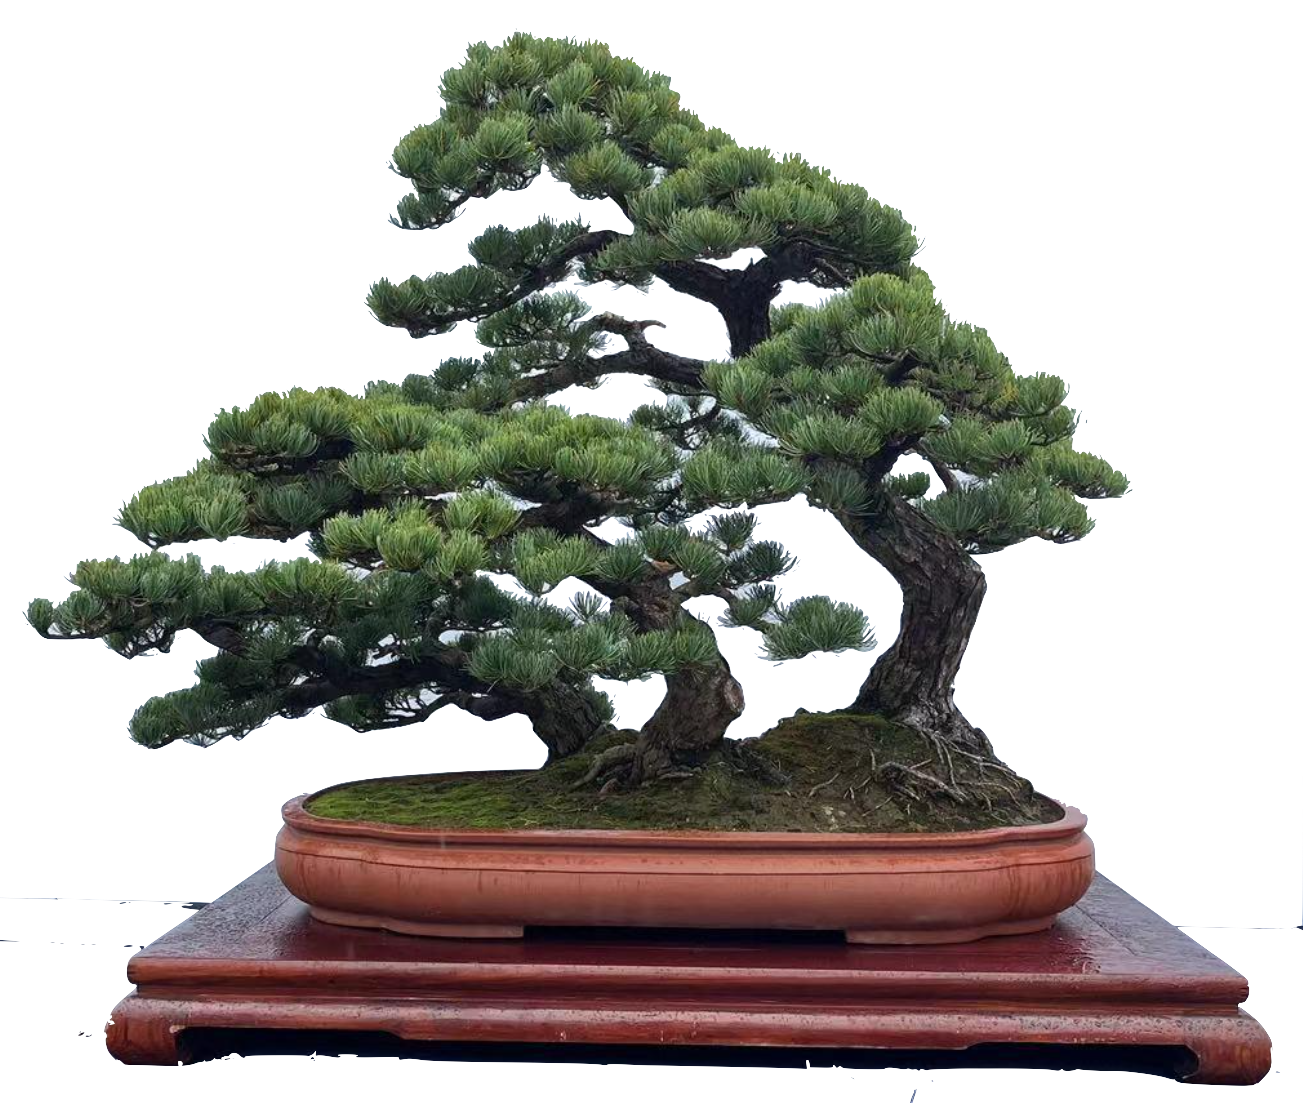
\includegraphics[width=0.7\columnwidth]{res/filler_a.png}
\end{center}
\columnbreak

